\section{Three Basic Waveforms and Why No Sine Wave?}
\label{sec:waveforms}

Sound chips in the 1980s generated three fundamental waveforms (Figure~\ref{fig:three-waves}) using simple digital circuits.

\begin{itemize}
  \item \textbf{Square wave.} Generated by a frequency divider.
  The chip counts system clock cycles and toggles between high and low voltage at a desired frequency.
  \item \textbf{Sawtooth wave.} Created with a digital accumulator.
  The accumulator repeatedly adds a fixed step.
  When it reaches the maximum, it resets instantly to zero.
  \item \textbf{Noise wave.} Produced by a linear feedback shift register (LFSR), a pseudo-random circuit that uses XOR feedback to generate a random stream of bits.
\end{itemize}

These three waveforms, requiring only a few logic gates and counters, became the building blocks of nearly all 8-bit game audio in the 1980s.

Although the sine wave is the most fundamental waveform in signal processing, it was absent from these chips.
Generating a sine wave was simply too expensive for 1980s hardware.

\begin{itemize}
  \item \textbf{Computational cost.} A sine wave requires trigonometric functions or Taylor-series expansion.
  A slow 4-bit or 8-bit CPU with no hardware multiplier could not perform such calculations in real time.
  \item \textbf{Hardware limitation.} A smooth sine wave needs a high-precision DAC.
  Most sound chips at that time had only primitive counter-based DACs, or no DAC at all---they produced step-like outputs rather than smooth curves.
  \item \textbf{Memory waste.} An alternative is to pre-compute sine values and store them in a lookup table (LUT), which would consume valuable ROM measured in kilobytes.
\end{itemize}

\begin{figure}[htbp]
  \centering
  \subfigure[Square wave.\label{fig:square}]{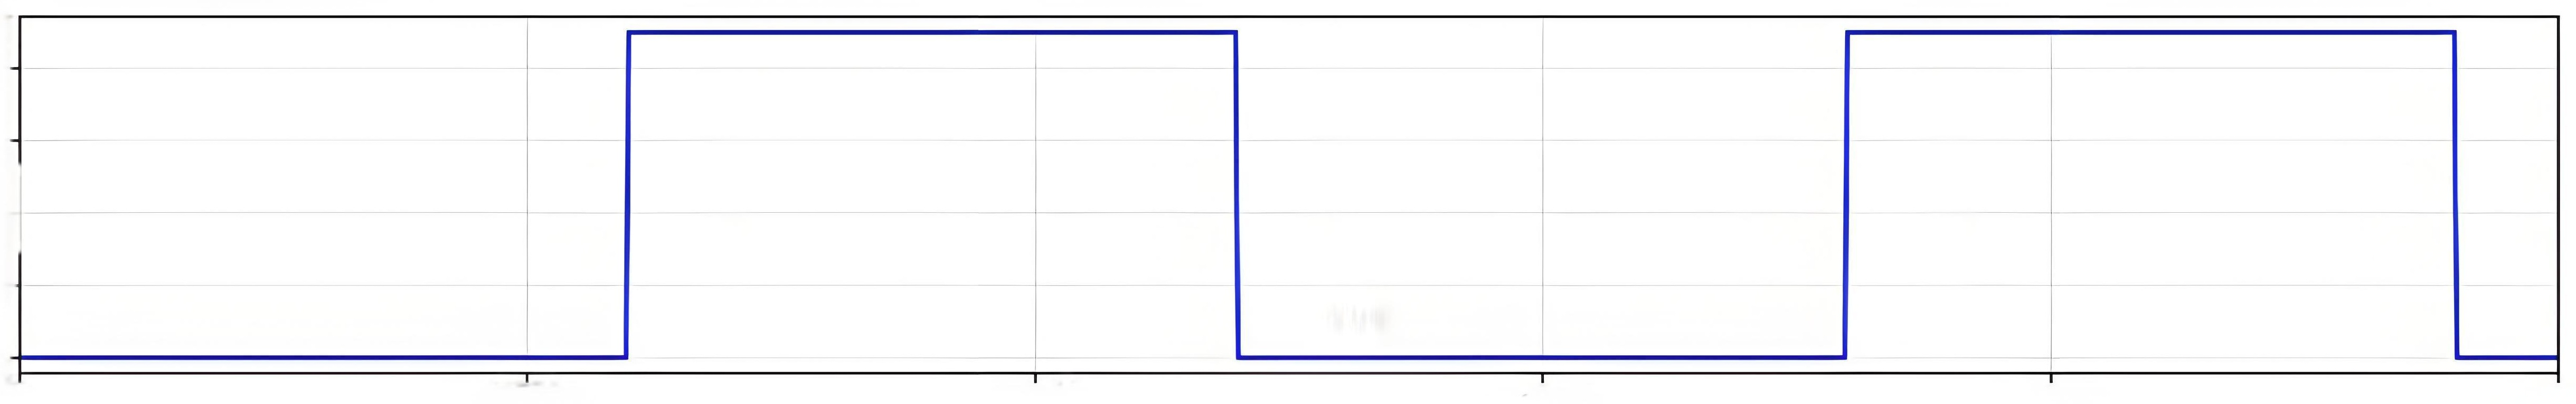
\includegraphics[width=0.32\linewidth]{pictures/square.png}}
  \hfill
  \subfigure[Sawtooth wave.\label{fig:sawtooth}]{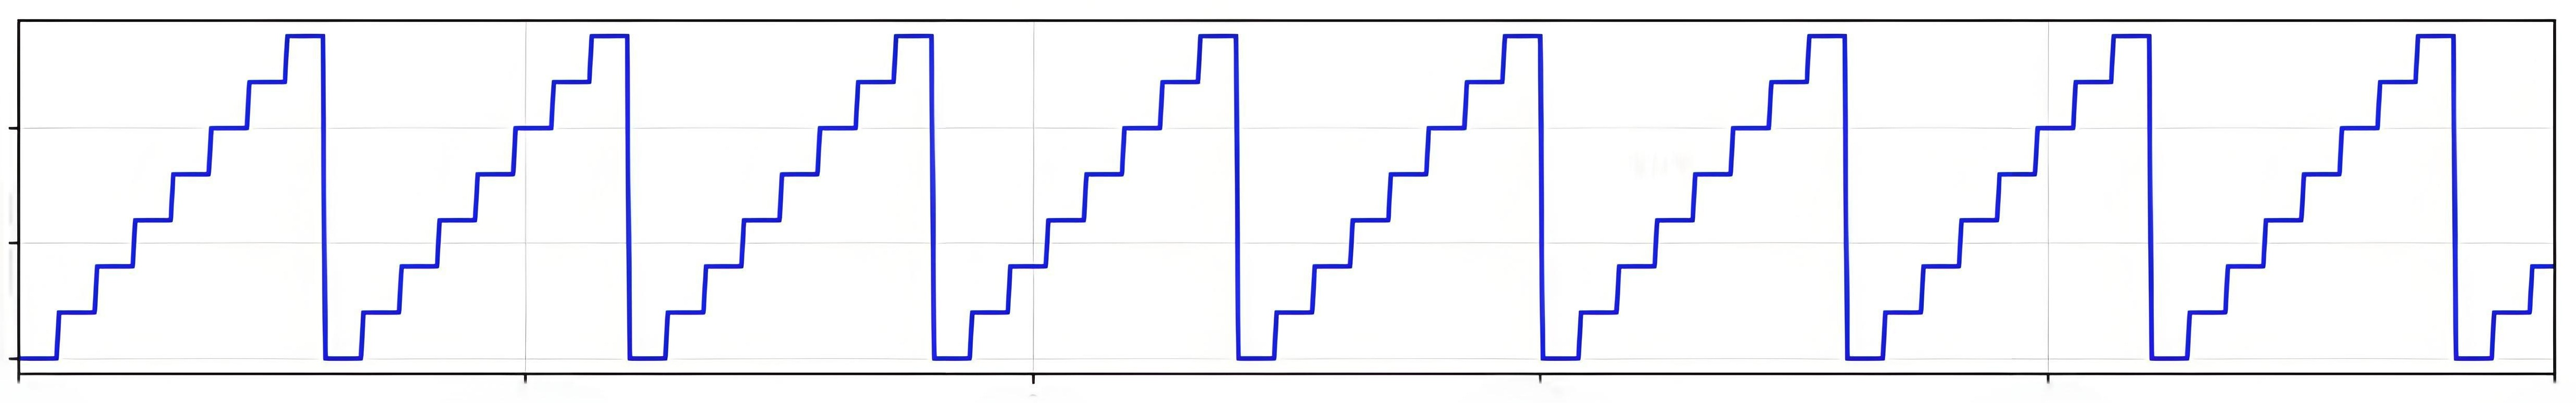
\includegraphics[width=0.32\linewidth]{pictures/sawtooth.png}}
  \hfill
  \subfigure[Noise wave.\label{fig:noise-wave}]{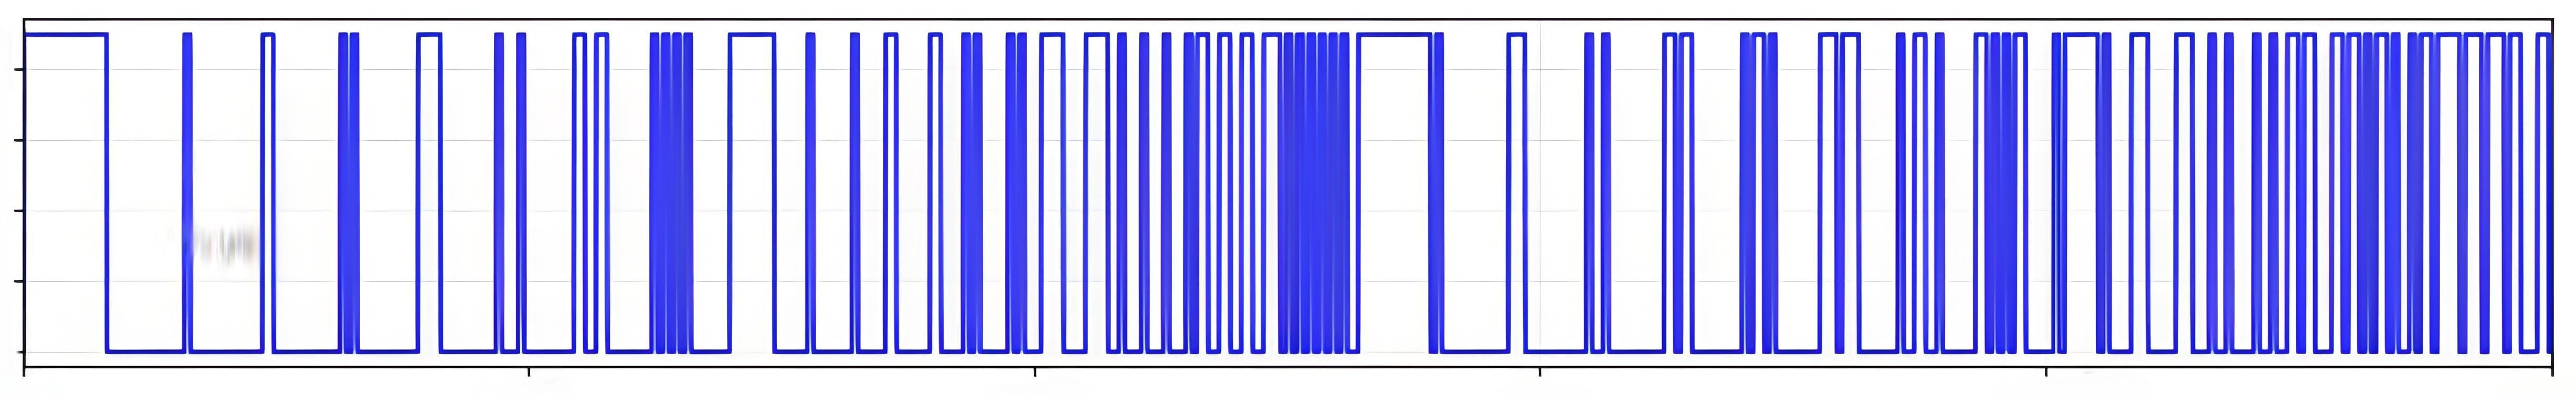
\includegraphics[width=0.32\linewidth]{pictures/noise.png}}
  \caption{Three basic waveforms.}
  \label{fig:three-waves}
\end{figure}
